\documentclass[12pt,letterpaper]{article}
% Some basic packages
\usepackage[utf8]{inputenc}
\usepackage[T1]{fontenc}
\usepackage{textcomp}
\usepackage{url}
\usepackage{graphicx}
\usepackage{float}
\usepackage{booktabs}
\usepackage{enumitem}
\usepackage{comment}

\pdfminorversion=7

% Don't indent paragraphs, leave some space between them
% \usepackage{parskip}

% Hide page number when page is empty
\usepackage{emptypage}
\usepackage{subcaption}
\usepackage{multicol}
\usepackage{xcolor}

% Other font I sometimes use.
% \usepackage{cmbright}

% Math stuff
\usepackage{amsmath, amsfonts, mathtools, amsthm, amssymb}
% Fancy script capitals
\usepackage{mathrsfs}
\usepackage{cancel}
% Bold math
\usepackage{bm}
% Some shortcuts
\newcommand\N{\ensuremath{\mathbb{N}}}
\newcommand\R{\ensuremath{\mathbb{R}}}
\newcommand\Z{\ensuremath{\mathbb{Z}}}
\renewcommand\O{\ensuremath{\emptyset}}
\newcommand\Q{\ensuremath{\mathbb{Q}}}
\newcommand\C{\ensuremath{\mathbb{C}}}
\newcommand{\genstirlingI}[3]{%
  \genfrac{[}{]}{0pt}{#1}{#2}{#3}%
}
\newcommand{\genstirlingII}[3]{%
  \genfrac{\{}{\}}{0pt}{#1}{#2}{#3}%
}
\newcommand{\stirlingI}[2]{\genstirlingI{}{#1}{#2}}
\newcommand{\dstirlingI}[2]{\genstirlingI{0}{#1}{#2}}
\newcommand{\tstirlingI}[2]{\genstirlingI{1}{#1}{#2}}
\newcommand{\stirlingII}[2]{\genstirlingII{}{#1}{#2}}
\newcommand{\dstirlingII}[2]{\genstirlingII{0}{#1}{#2}}
\newcommand{\tstirlingII}[2]{\genstirlingII{1}{#1}{#2}}

% Easily typeset systems of equations (French package)
\usepackage{systeme}

% Put x \to \infty below \lim
\let\svlim\lim\def\lim{\svlim\limits}

%Make implies and impliedby shorter
\let\implies\Rightarrow
\let\impliedby\Leftarrow
\let\iff\Leftrightarrow
\let\epsilon\varepsilon

% Add \contra symbol to denote contradiction
\usepackage{stmaryrd} % for \lightning
\newcommand\contra{\scalebox{1.5}{$\lightning$}}

% \let\phi\varphi

% Command for short corrections
% Usage: 1+1=\correct{3}{2}

\definecolor{correct}{HTML}{009900}
\newcommand\correct[2]{\ensuremath{\:}{\color{red}{#1}}\ensuremath{\to }{\color{correct}{#2}}\ensuremath{\:}}
\newcommand\green[1]{{\color{correct}{#1}}}

% horizontal rule
\newcommand\hr{
    \noindent\rule[0.5ex]{\linewidth}{0.5pt}
}

% hide parts
\newcommand\hide[1]{}

% si unitx
\usepackage{siunitx}
\sisetup{detect-family}

% Environments
\makeatother
% For box around Definition, Theorem, \ldots
\usepackage{mdframed}
\mdfsetup{skipabove=1em,skipbelow=0em}
\theoremstyle{definition}
\newmdtheoremenv[nobreak=true]{definition}{Definition}
\newmdtheoremenv[nobreak=true]{result}{Result}
\newmdtheoremenv[nobreak=true]{lemma}{Lemma}
\newmdtheoremenv[nobreak=true]{proposition}{Proposition}
\newmdtheoremenv[nobreak=true]{theorem}{Theorem}
\newmdtheoremenv[nobreak=true]{law}{Law}
\newmdtheoremenv[nobreak=true]{postulate}{Postulate}
\newmdtheoremenv{conclusion}{Conclusion}
\newmdtheoremenv{addition}{Addition}
\newmdtheoremenv{presumption}{Presumption}
\newtheorem*{repetition}{Repetition}
\newtheorem*{interlude}{Interlude}
\newtheorem*{notation}{Notation}
\newtheorem*{observation}{Observation}
\newtheorem*{exercise}{Exercise}
\newtheorem*{remark}{Remark}
\newtheorem*{practice}{Practice}
\newtheorem*{problem}{Problem}
\newtheorem*{term}{Terminology}
\newtheorem*{application}{Application}
\newtheorem*{eg}{Example}
\newtheorem*{question}{Question}

% \newmdtheoremenv[nobreak=true]{definition}{Definition}
% \newtheorem*{eg}{Example}
% \newtheorem*{notation}{Notation}
% \newtheorem*{previouslyseen}{As previously seen}
% \newtheorem*{remark}{Remark}
% \newtheorem*{note}{Note}
% \newtheorem*{problem}{Problem}
% \newtheorem*{observe}{Observe}
% \newtheorem*{property}{Property}
% \newtheorem*{intuition}{Intuition}
% \newmdtheoremenv[nobreak=true]{prop}{Proposition}
% \newmdtheoremenv[nobreak=true]{theorem}{Theorem}
\newmdtheoremenv[nobreak=true]{corollary}{Corollary}

% End example and intermezzo environments with a small diamond (just like proof
% environments end with a small square)
\usepackage{etoolbox}
\AtEndEnvironment{eg}{\null\hfill$\diamond$}%
\AtEndEnvironment{interlude}{\null\hfill$\diamond$}%
% \AtEndEnvironment{opmerking}{\null\hfill$\diamond$}%

% Fix some spacing
% http://tex.stackexchange.com/questions/22119/how-can-i-change-the-spacing-before-theorems-with-amsthm
\makeatletter
\def\thm@space@setup{%
  \thm@preskip=\parskip \thm@postskip=0pt
}


% Exercise 
% Usage:
% \oefening{5}
% \suboefening{1}
% \suboefening{2}
% \suboefening{3}
% gives
% Oefening 5
%   Oefening 5.1
%   Oefening 5.2
%   Oefening 5.3
\newcommand{\prac}[1]{%
    \def\@practice{#1}%
    \subsection*{Practice #1}
}

\newcommand{\subprac}[1]{%
    \subsubsection*{Practice \@practice.#1}
}


% \lecture starts a new lecture (les in dutch)
%
% Usage:
% \lecture{1}{di 12 feb 2019 16:00}{Inleiding}
%
% This adds a section heading with the number / title of the lecture and a
% margin paragraph with the date.

% I use \dateparts here to hide the year (2019). This way, I can easily parse
% the date of each lecture unambiguously while still having a human-friendly
% short format printed to the pdf.

\usepackage{xifthen}
\def\testdateparts#1{\dateparts#1\relax}
\def\dateparts#1 #2 #3 #4 #5\relax{
    \marginpar{\small\textsf{\mbox{#1 #2 #3 #5}}}
}

\def\@lecture{}%
\newcommand{\lecture}[3]{
    \ifthenelse{\isempty{#3}}{%
        \def\@lecture{Lecture #1}%
    }{%
        \def\@lecture{Lecture #1: #3}%
    }%
    \subsection*{\@lecture}
    \marginpar{\small\mbox{#2}}
}



% These are the fancy headers
% \usepackage{fancyhdr}
% \pagestyle{fancy}

% LE: left even
% RO: right odd
% CE, CO: center even, center odd
% My name for when I print my lecture notes to use for an open book exam.
% \fancyhead[LE,RO]{Gilles Castel}

% \fancyhead[RO,LE]{\@lecture} % Right odd,  Left even
% \fancyhead[RE,LO]{}          % Right even, Left odd

% \fancyfoot[RO,LE]{\thepage}  % Right odd,  Left even
% \fancyfoot[RE,LO]{}          % Right even, Left odd
% \fancyfoot[C]{\leftmark}     % Center

% \makeatother

% Shortcut for nth numbering
\usepackage[super]{nth}

% Todonotes and inline notes in fancy boxes
\usepackage{todonotes}
\usepackage{tcolorbox}

% Make boxes breakable
\tcbuselibrary{breakable}

% Verbetering is correction in Dutch
% Usage: 
% \begin{verbetering}
%     Lorem ipsum dolor sit amet, consetetur sadipscing elitr, sed diam nonumy eirmod
%     tempor invidunt ut labore et dolore magna aliquyam erat, sed diam voluptua. At
%     vero eos et accusam et justo duo dolores et ea rebum. Stet clita kasd gubergren,
%     no sea takimata sanctus est Lorem ipsum dolor sit amet.
% \end{verbetering}
\newenvironment{correction}{\begin{tcolorbox}[
    arc=0mm,
    colback=white,
    colframe=green!60!black,
    title=Correction,
    fonttitle=\sffamily,
    breakable
]}{\end{tcolorbox}}

% Noot is note in Dutch. Same as 'verbetering' but color of box is different
\newenvironment{note}[1]{\begin{tcolorbox}[
    arc=0mm,
    colback=white,
    colframe=white!60!black,
    title=#1,
    fonttitle=\sffamily,
    breakable
]}{\end{tcolorbox}}




% Figure support as explained in my blog post.
\usepackage{import}
\usepackage{pdfpages}
\usepackage{transparent}

% Fix some stuff
% %http://tex.stackexchange.com/questions/76273/multiple-pdfs-with-page-group-included-in-a-single-page-warning
\pdfsuppresswarningpagegroup=1


% text and symbol support
\usepackage[normalem]{ulem}
\useunder{\uline}{\ul}{}

% formatting support
\usepackage{framed}
\usepackage[page]{appendix}
\usepackage{authblk}

% figure support
\newcommand{\incfig}[1]{%
  \def\svgwidth{\columnwidth}
  \import{./figures/}{#1.pdf_tex}
}
\usepackage{pgfplots}
\pgfplotsset{width=7cm,compat=1.18}
\usepackage[section]{placeins}
\captionsetup{subrefformat=parens}

% table support
\usepackage{longtable}
\usepackage{array}

% bibliography support
\usepackage[backend=biber,style=apa]{biblatex}
\addbibresource{~/Library/texmf/bibtex/bib/Zotero.bib}

% additional packages
\usepackage{lipsum, verbatim}
\usepackage{hyperref}
\usepackage{bookmark}

% matrix stretching macro modification
% \makeatletter
% \renewcommand*\env@matrix[1][\arraystretch]{%
%   \edef\arraystretch{#1}%
%   \hskip -\arraycolsep
%   \let\@ifnextchar\new@ifnextchar
%   \array{*\c@MaxMatrixCols c}}
% \makeatother

% My name
\author[1]{Annais Gangolf\thanks{agangolf@haverford.edu}}
\author[1]{Devansh Goyal\thanks{dgoyal@haverford.edu}}
\author[1]{Samuel E. Ross\thanks{seross@haverford.edu}}
  \affil[1]{Economics Research Club, Haverford College, Haverford, PA 19041, USA}
\date{\today}
\setcounter{Maxaffil}{0}
\renewcommand\Affilfont{\itshape\small}



\title{Summary of Replication Efforts for Section IV.A of Chetty et al.’s ``The Economic Impacts of COVID-19: Evidence from a New Public Database Built Using Private Sector Data''}
\begin{document}
  \maketitle
  \section{Introduction}
    The Haverford Economics Research Club is a student group at Haverford College which offers students the opportunity to learn about the structure and execution of economic research. In service of this goal, we are beginning to write an extension of Section IV.A of "The Economic Impacts of COVID-19: Evidence from a New Public Database Built Using Private Sector Data" \parencite{Chetty2020} the extension of which concerns the effect of varied reopening strategies (i.e., multi-phase reopenings, rather than the original single-event analysis) on consumer spending, employment, and business openings.  We have begun our work by attempting to replicate the paper’s original findings.
  \section{Replication}
    The figures listed below are our attempt to replicate Table 3 columns (1), (2), (3), (4), (5), (6), (7), (8), (9), (10) in addition to Figure 12b, Figure 12c, and Figure 12d.  In each of the OLS regressions, doesOpen (or ‘opener’) is an indicator variable for whether the state is a treatment or control, afterEvent (or ‘openTime’) is an indicator variable for whether the observation is past the relevant reopening date, and isOpen (or ‘reopened’) is an interaction term between the preceding two variables. 
      
      \subsection{Consumer Spending}
        Raw data obtained from the Opportunity Insights GitHub page were processed by collapsing the frequency to weekly by eliminating all non-Sunday observations.  This method was used due to the raw data’s format as a 7-day moving average.  All other variable coding and processing was consistent with the working paper’s specifications.
        \begin{figure}[!ht]
          \centering
          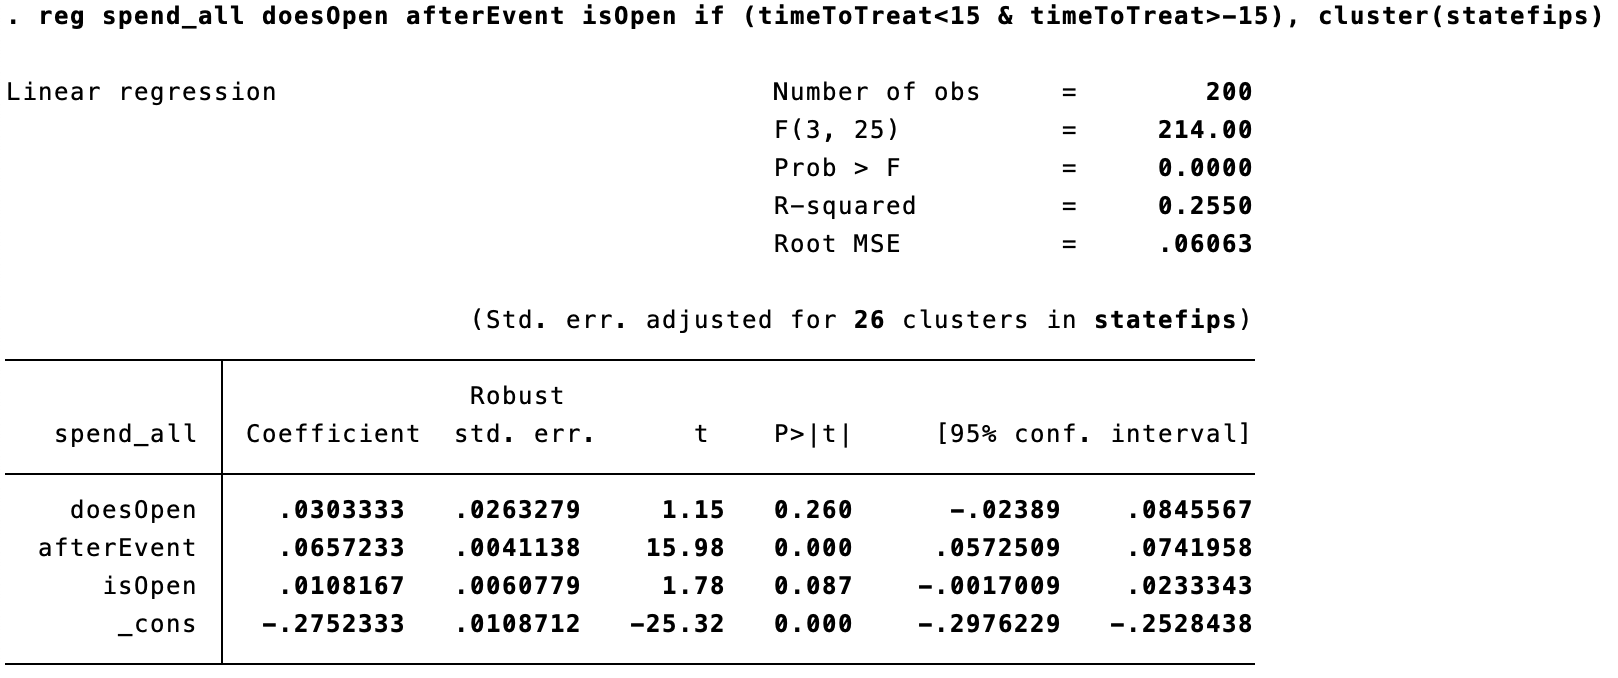
\includegraphics[width=0.8\textwidth]{figures/spend_all_2wk.png}
          \caption{OLS Regression performed on spend\_all in doesOpen, afterEvent, and isOpen over 2-week horizon.  Predicts 1.08 p.p. increase in consumer spending with reopening.}
          \label{fig:figures-spend_all_2wk-png}
        \end{figure}
        \begin{figure}[!ht]
          \centering
          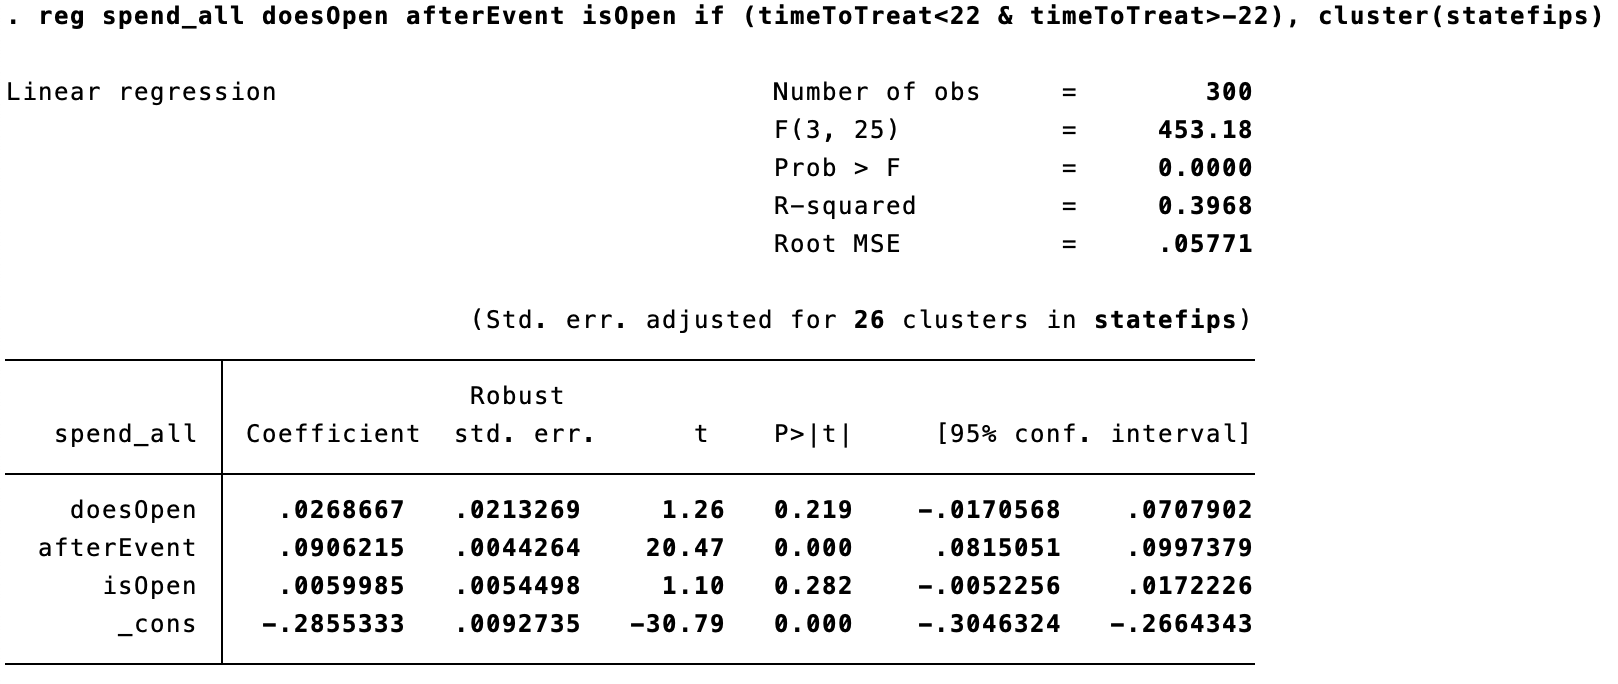
\includegraphics[width=0.8\textwidth]{figures/spend_all_3wk.png}
          \caption{OLS Regression performed on spend\_all in doesOpen, afterEvent, and isOpen over 3-week horizon.  Predicts 0.59 p.p. increase in consumer spending with reopening.}
          \label{fig:figures-spend_all_3wk-png}
        \end{figure}
        \begin{figure}[!ht]
          \centering
          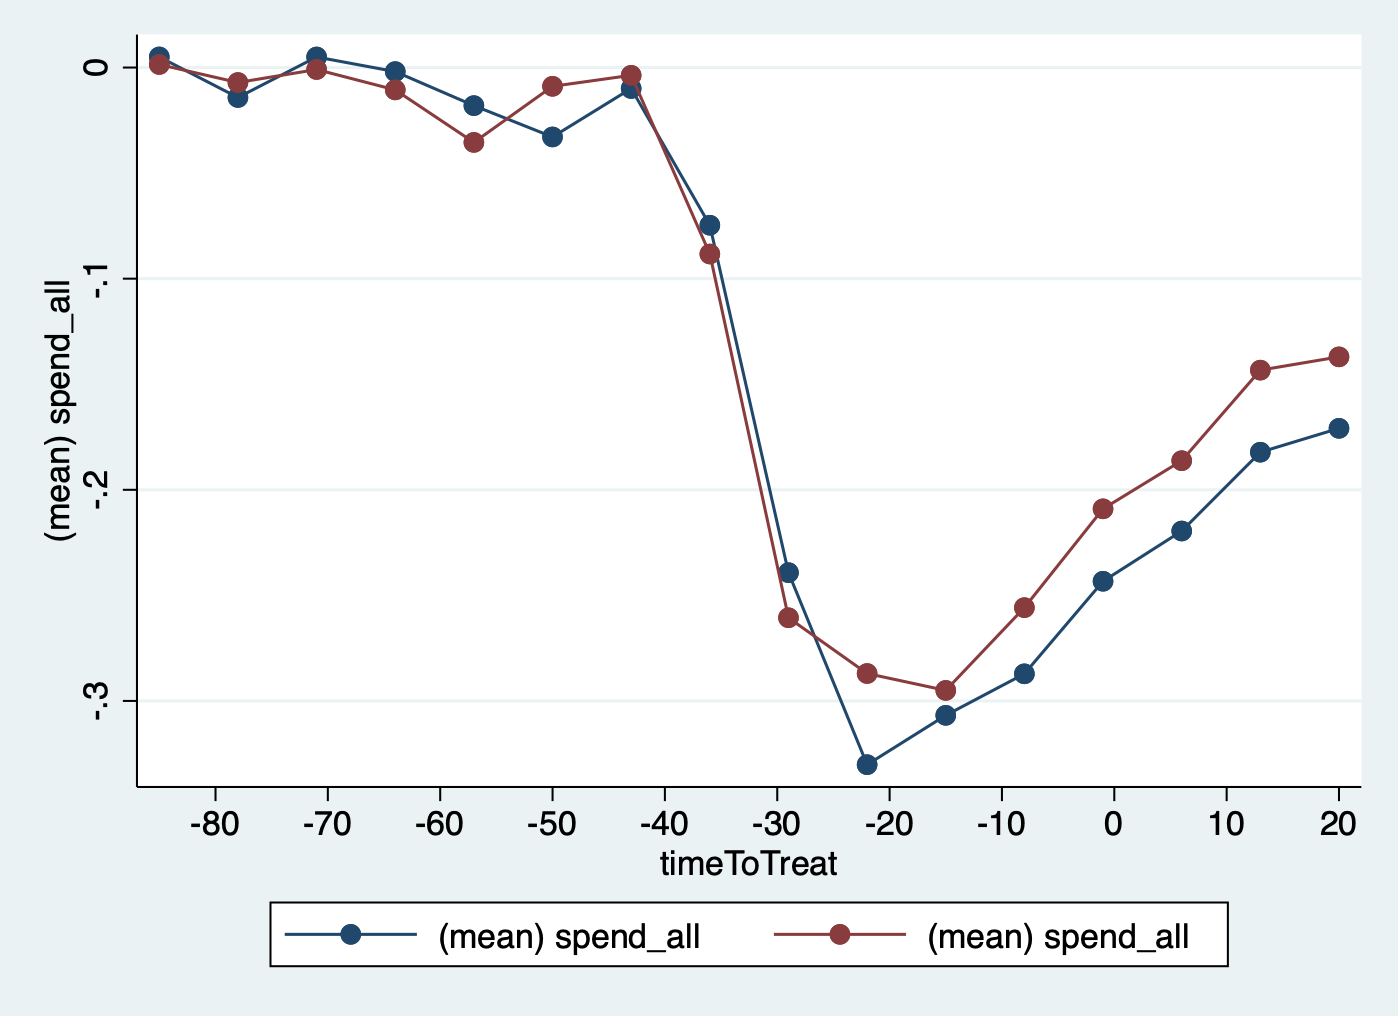
\includegraphics[width=0.8\textwidth]{figures/spend_all_graph.png}
\caption{To create this graph, the spend\_all series for the April 24th reopening date was redefined as the Thursday value, rather than the Sunday value, in order to put our event timing variable, timeToTreat, into phase across the three treatment groups.  These series were then aggregated and collapsed by treatment vs. control status and time relative to treatment (timeToTreat).}
          \label{fig:figures-spend_all_graph-png}
        \end{figure}
        \clearpage
      \subsection{Employment}
Raw data obtained from the Opportunity Insights GitHub page were processed by collapsing the frequency to weekly by taking the average of each Sunday–Saturday week and attributing this mean to the Sunday’s date.  All other variable coding and processing was consistent with the working paper’s specifications.
        \begin{figure}[!ht]
          \centering
          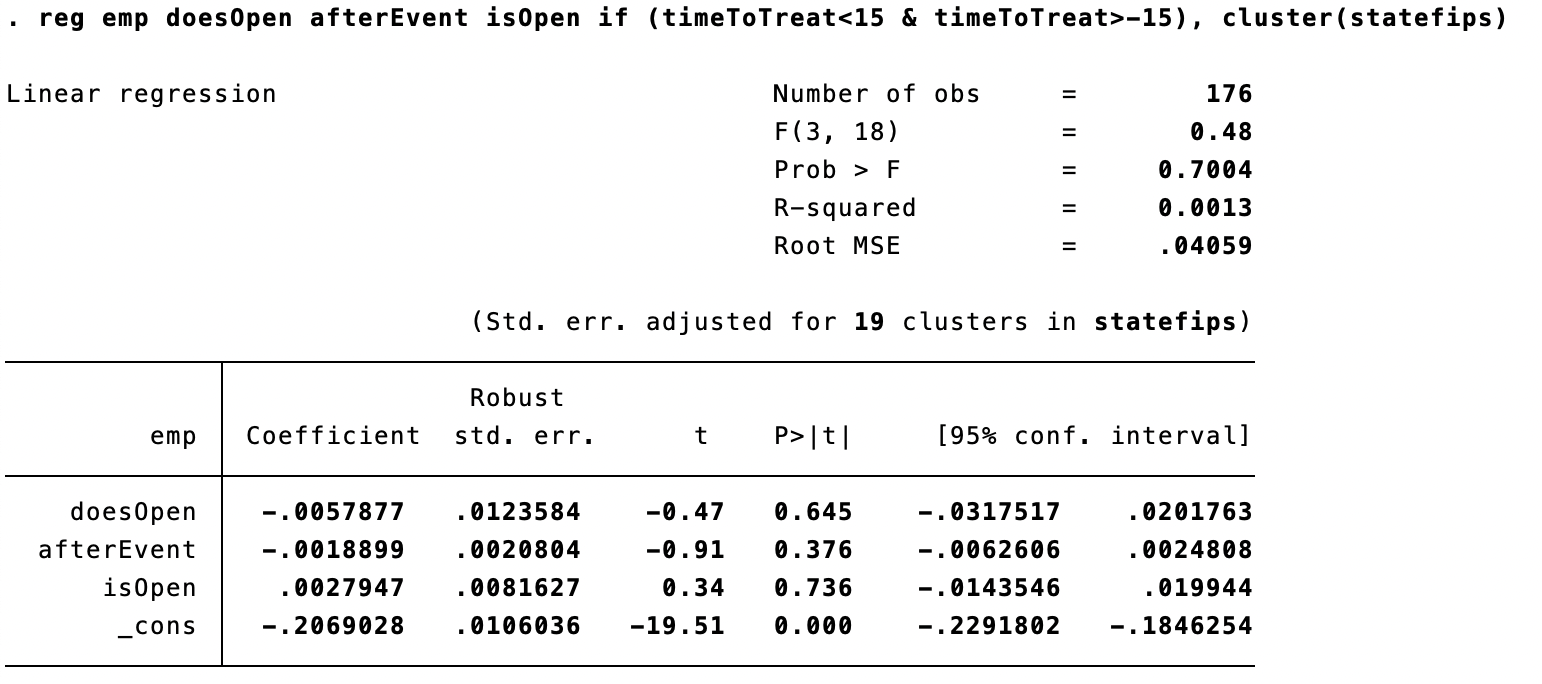
\includegraphics[width=0.8\textwidth]{figures/emp_2wk.png}
\caption{OLS Regression performed on emp in doesOpen, afterEvent, and isOpen over 2-week horizon.  Predicts 0.27 p.p. increase in employment with reopening.}
          \label{fig:figures-emp_2wk-png}
        \end{figure}
        \begin{figure}[!ht]
          \centering
          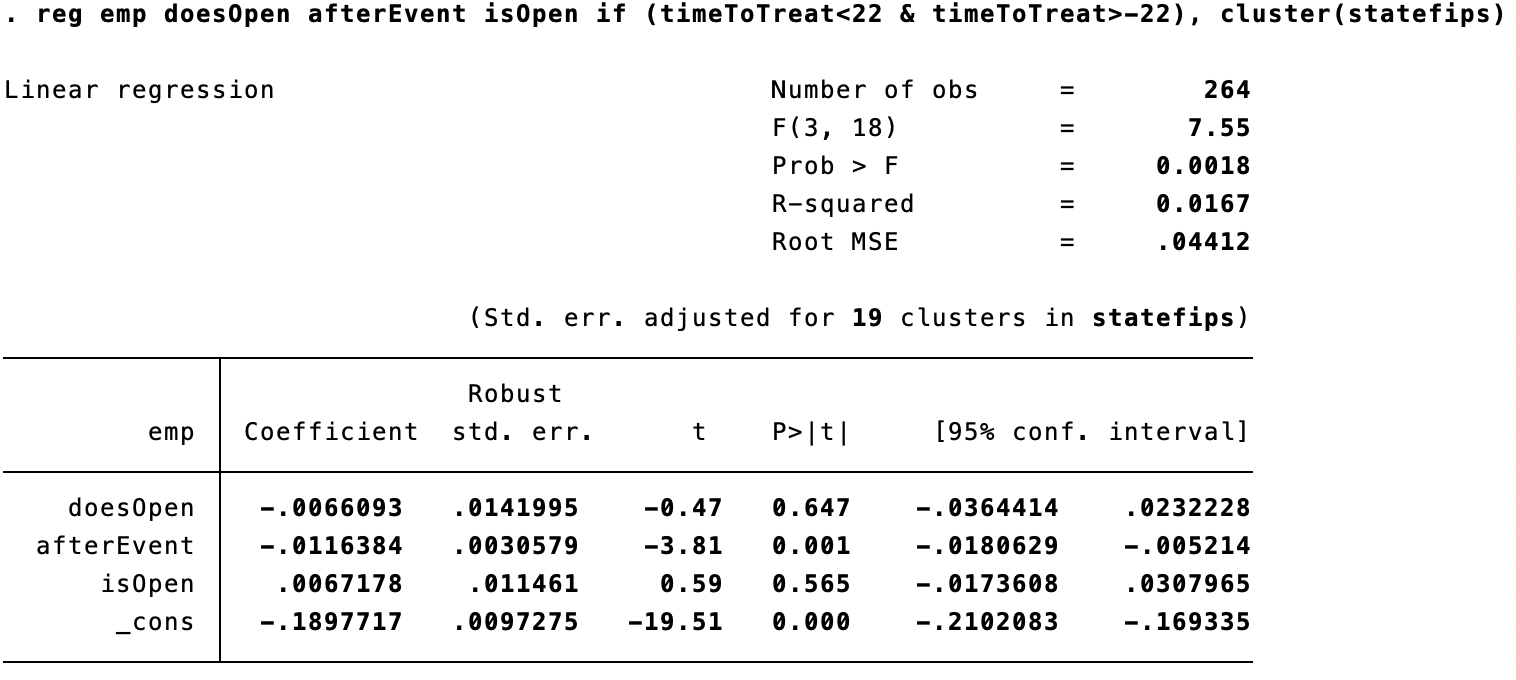
\includegraphics[width=0.8\textwidth]{figures/emp_3wk.png}
\caption{OLS Regression performed on emp in doesOpen, afterEvent, and isOpen over 3-week horizon.  Predicts 0.67 p.p. increase in employment with reopening.}
          \label{fig:figures-emp_3wk-png}
        \end{figure}
        \begin{figure}[!ht]
          \centering
          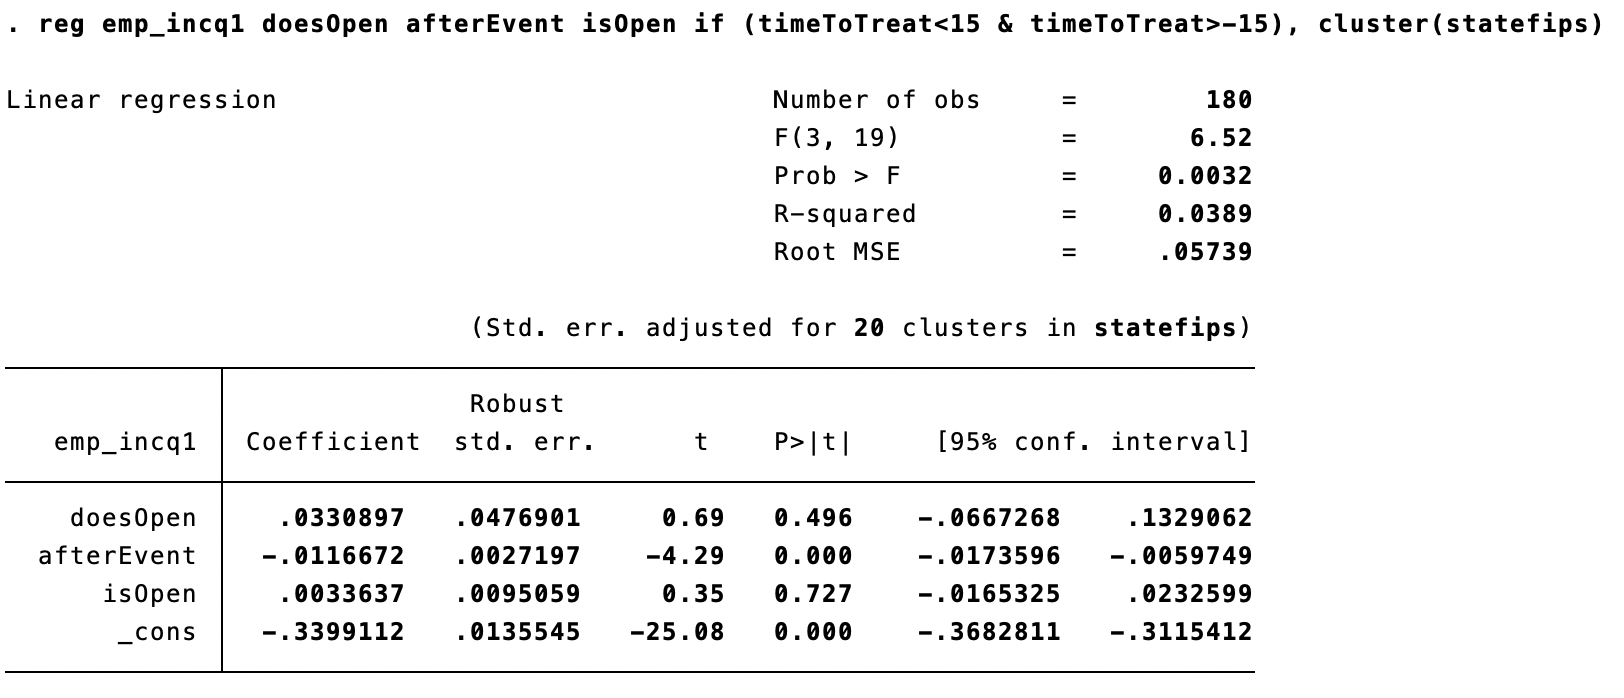
\includegraphics[width=0.8\textwidth]{figures/emp_incq1.png}
\caption{OLS Regression performed on emp\_incq1 in doesOpen, afterEvent, and isOpen over 2-week horizon.  Predicts 0.33 p.p. increase in first-income-quartile employment with reopening.}
          \label{fig:figures-emp_incq1-png}
        \end{figure}
        \begin{figure}[!ht]
          \centering
          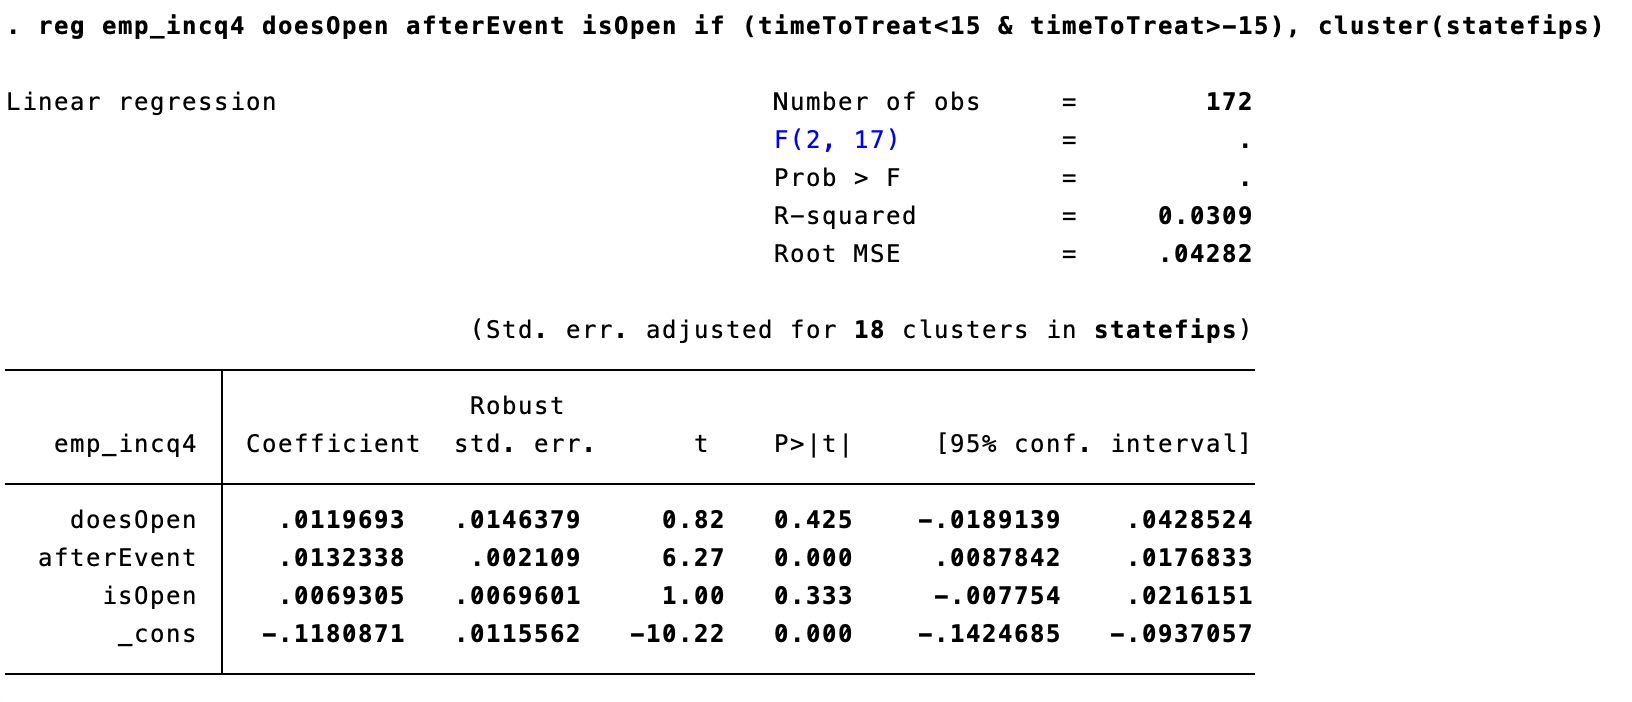
\includegraphics[width=0.8\textwidth]{figures/emp_incq4.png}
\caption{OLS Regression performed on emp\_incq4 in doesOpen, afterEvent, and isOpen over 2-week horizon.  Predicts 0.69 p.p. increase in fourth-income-quartile employment with reopening.}
          \label{fig:figures-emp_incq4-png}
        \end{figure}
        \begin{figure}[!ht]
          \centering
          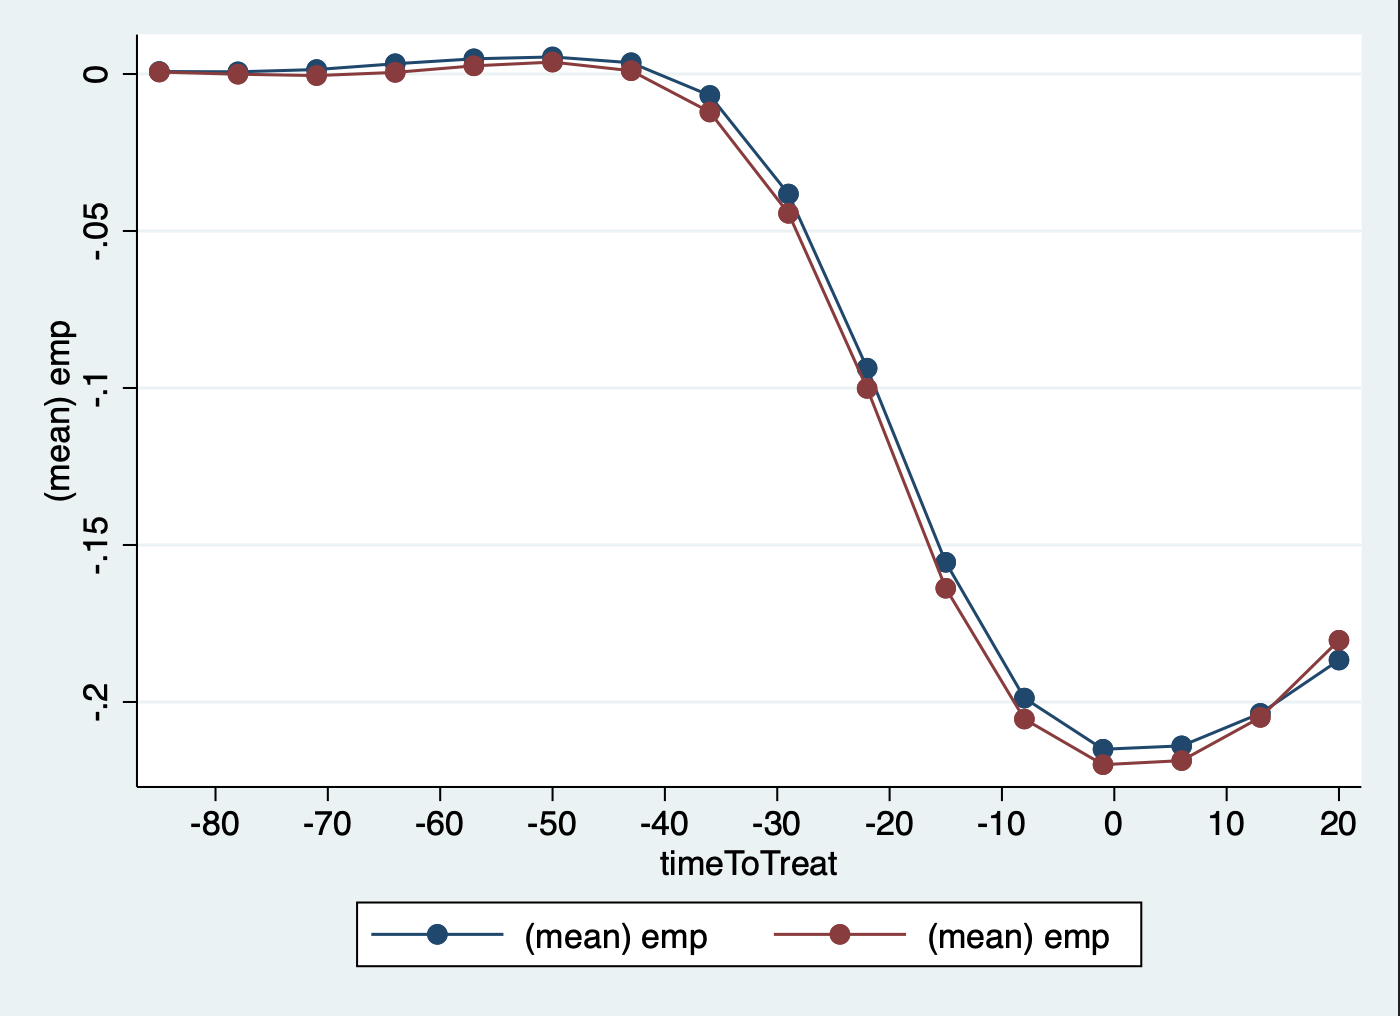
\includegraphics[width=0.8\textwidth]{figures/emp_graph.png}
\caption{To create this graph, the emp series for the April 24th reopening date was redefined using a Thursday-–Wednesday week, in order to put our event timing variable, timeToTreat, into phase across the three treatment groups.  These series were then aggregated and collapsed by treatment vs. control status and time relative to treatment (timeToTreat).}
          \label{fig:figures-emp_graph-png}
        \end{figure}
        \clearpage
      \subsection{Small Businesses}
        Raw data obtained from the Opportunity Insights GitHub page were processed by collapsing the frequency to weekly by eliminating all non-Sunday observations.  This method was used due to the raw data’s format as a 7-day moving average.  All other variable coding and processing was consistent with the working paper’s specifications.
        \begin{figure}[!ht]
          \centering
          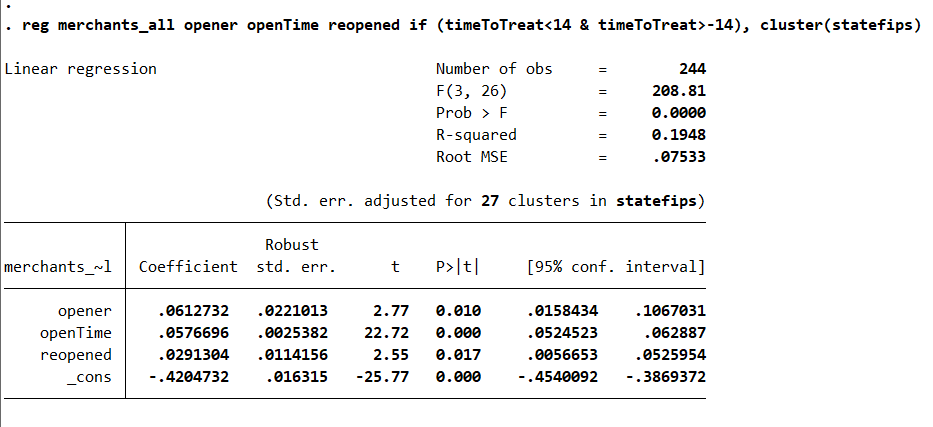
\includegraphics[width=0.8\textwidth]{figures/merchants_all_2wk.png}
\caption{OLS Regression performed on merchants\_all in opener, openTime, and reopened over 2-week horizon.  Predicts 2.91 p.p. increase in open small businesses with reopening.}
          \label{fig:figures-merchants_all_2wk-png}
        \end{figure}
        \begin{figure}[!ht]
          \centering
          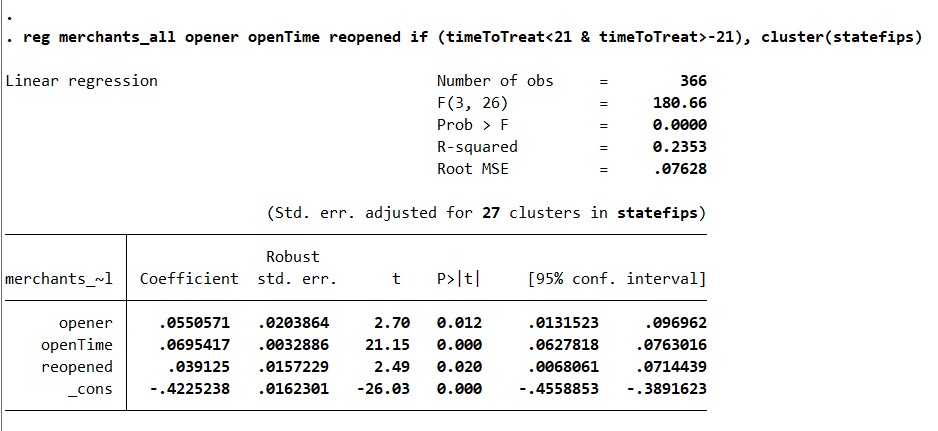
\includegraphics[width=0.8\textwidth]{figures/merchants_all_3wk.png}
\caption{OLS Regression performed on merchants\_all in opener, openTime, and reopened over 3-week horizon.  Predicts 3.91 p.p. increase in open small businesses with reopening.}
          \label{fig:figures-merchants_all_3wk-png}
        \end{figure}
        \begin{figure}[!ht]
          \centering
          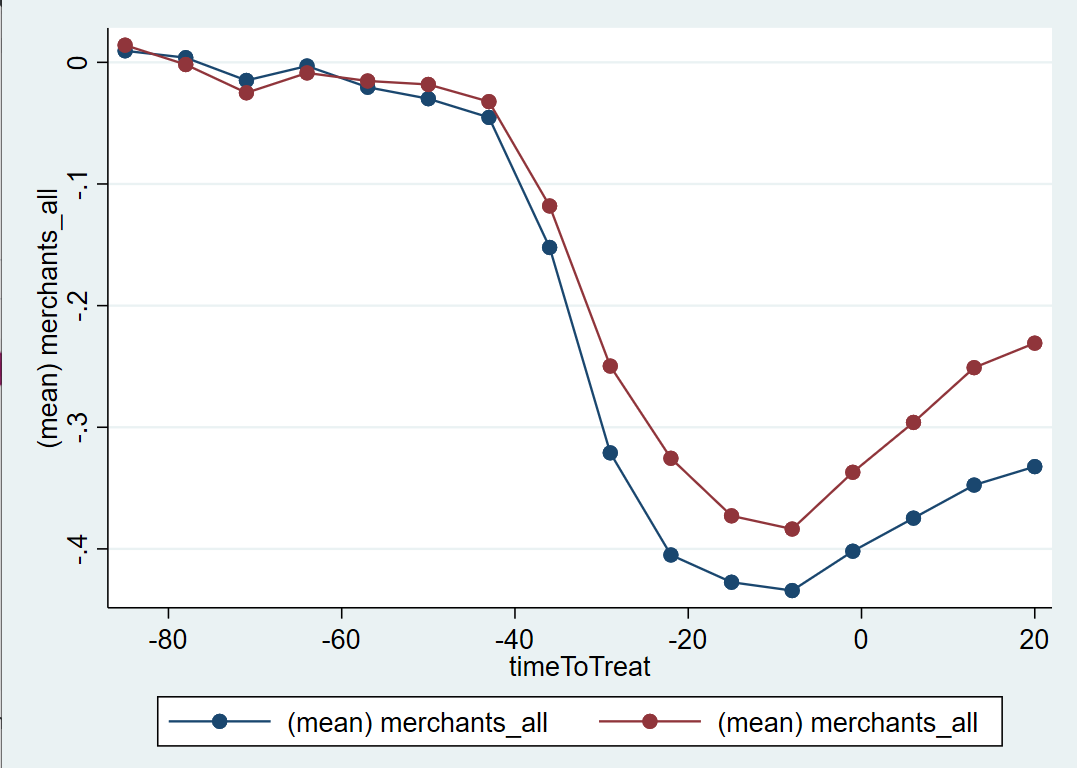
\includegraphics[width=0.8\textwidth]{figures/merchants_all_graph.png}
\caption{To create this graph, the merchants\_all series for the April 24th reopening date was redefined as the Thursday value, rather than the Sunday value, in order to put our event timing variable, timeToTreat, into phase across the three treatment groups.  These series were then aggregated and collapsed by treatment vs. control status and time relative to treatment (timeToTreat).}
          \label{fig:figures-merchants_all_graph-png}
        \end{figure}
        \clearpage
      \subsection{Mobility}
        Raw data obtained from the Opportunity Insights GitHub page were processed by collapsing the frequency to weekly by eliminating all non-Sunday observations.  This method was used due to the raw data’s format as a 7-day moving average.  All other variable coding and processing was consistent with the working paper’s specifications.
        \begin{figure}[!ht]
          \centering
          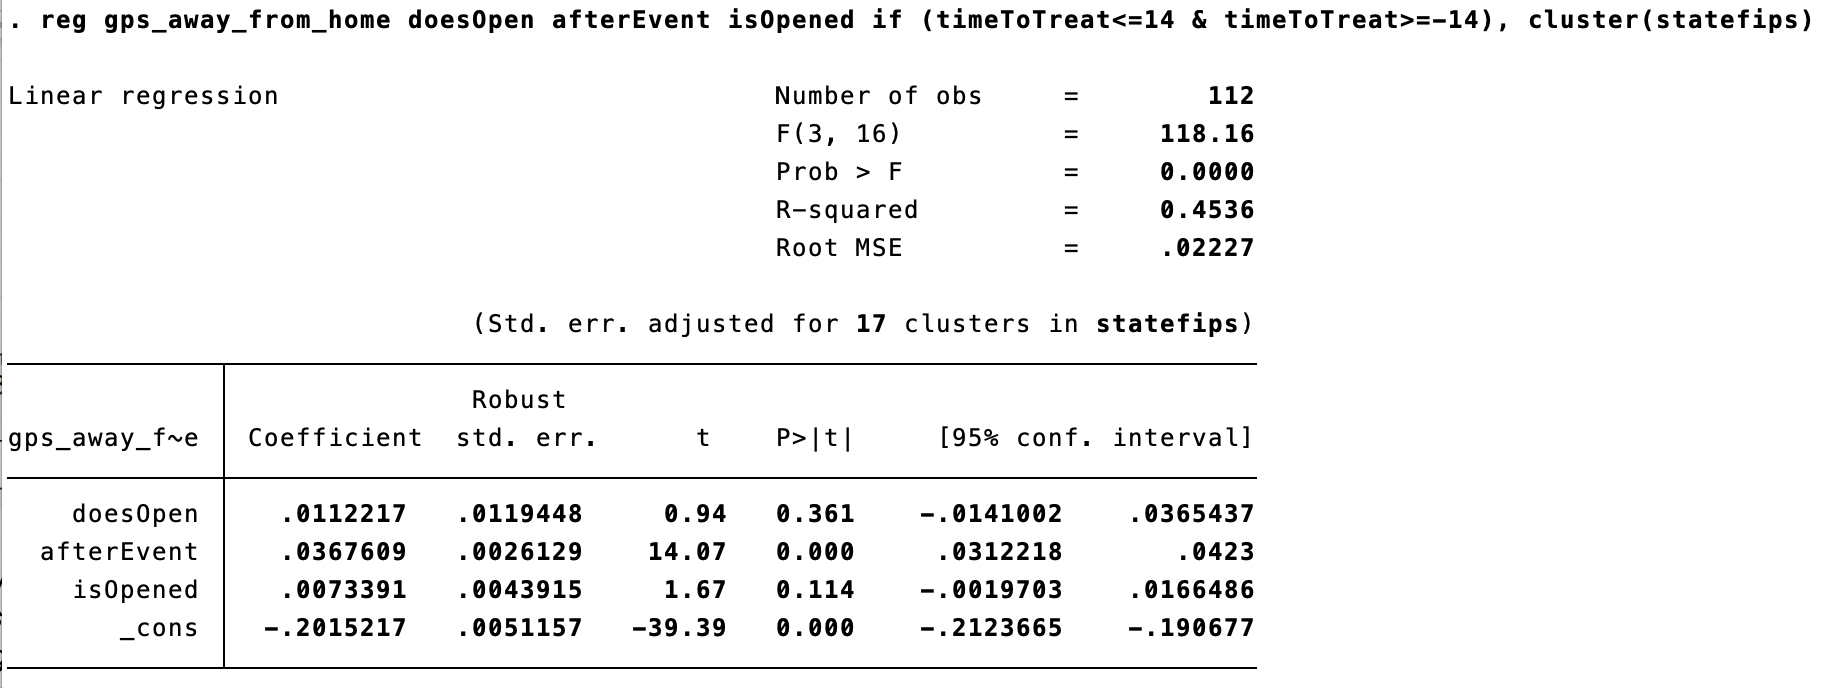
\includegraphics[width=0.8\textwidth]{figures/gps_2wk.png}
          \caption{OLS Regression performed on gps\_away\_from\_home in doesOpen, afterEvent, and isOpen over 2-week horizon.  Predicts 0.73 p.p. increase in consumer spending with reopening.}
          \label{fig:figures-gps_2wk-png}
        \end{figure}
        \begin{figure}[!ht]
          \centering
          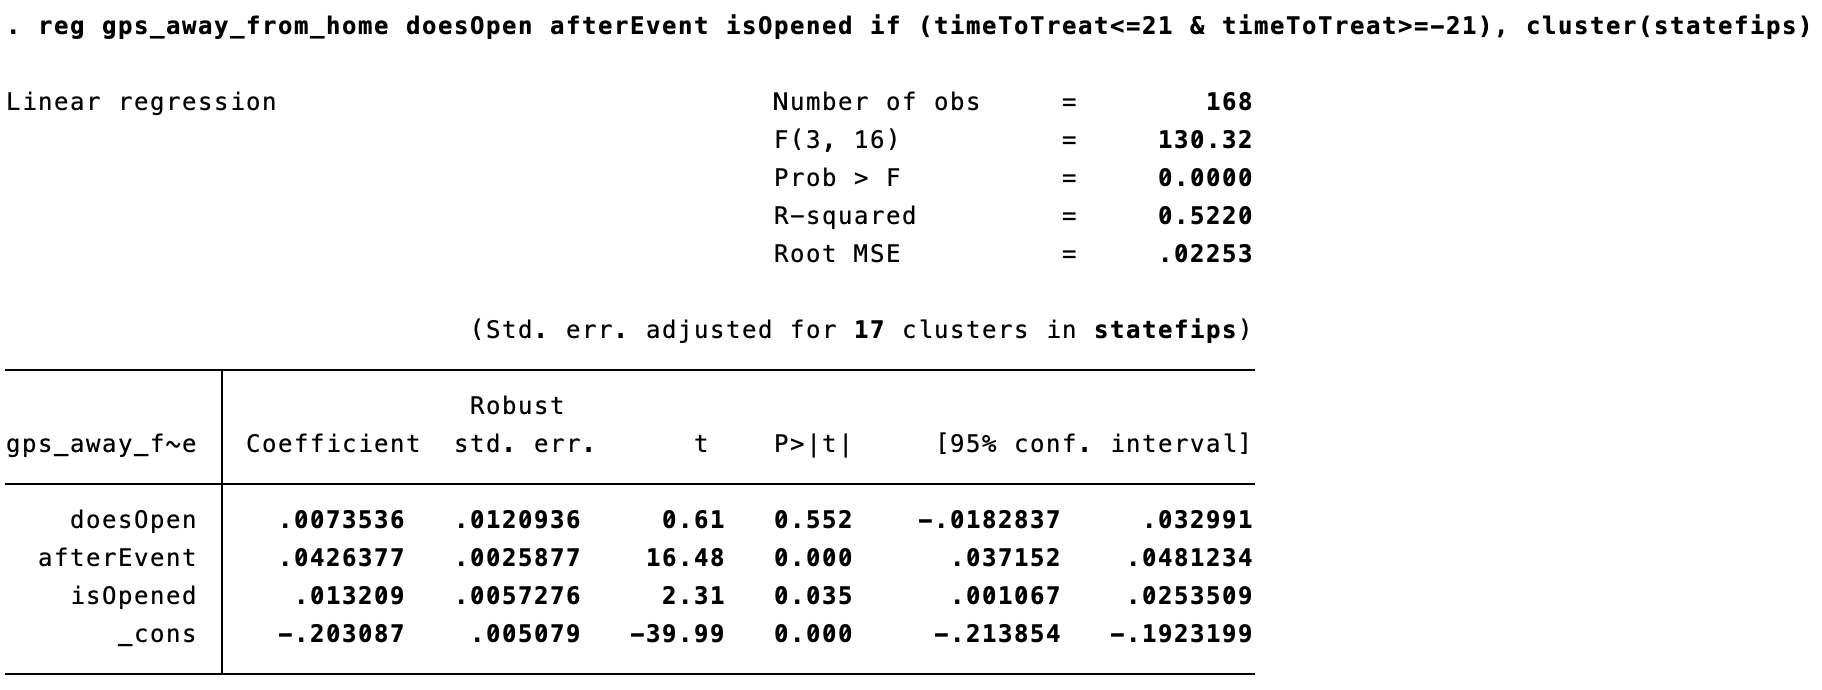
\includegraphics[width=0.8\textwidth]{figures/gps_3wk.png}
          \caption{OLS Regression performed on gps\_away\_from\_home in doesOpen, afterEvent, and isOpen over 3-week horizon.  Predicts 1.32 p.p. increase in consumer spending with reopening.}
          \label{fig:figures-gps_3wk-png}
        \end{figure}  
        \begin{figure}[!ht]
          \centering
          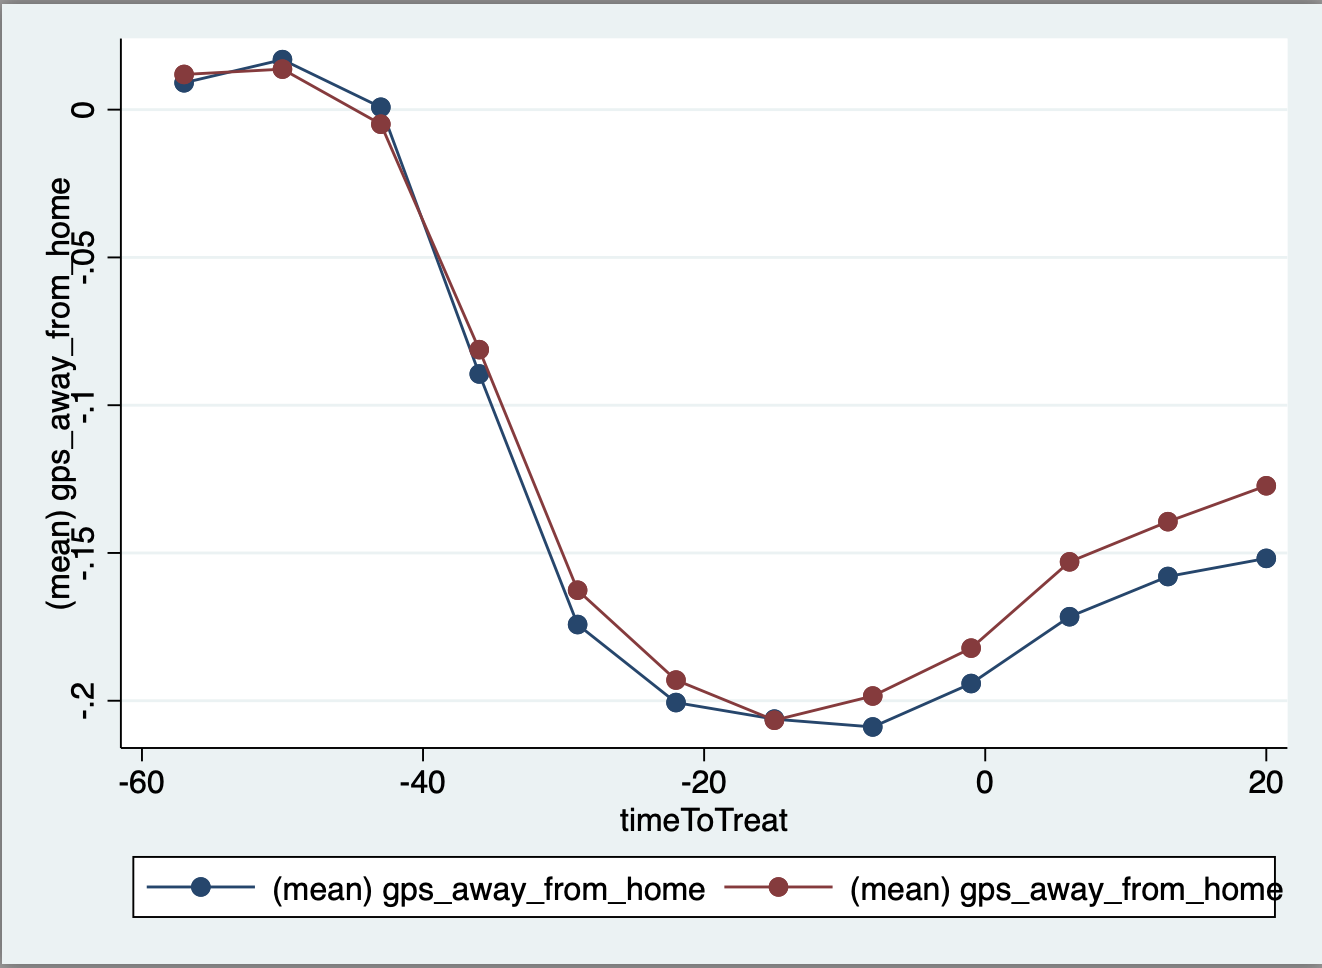
\includegraphics[width=0.8\textwidth]{figures/gps_graph.png}
\caption{To create this graph, the gps\_away\_from\_home series for the April 24th reopening date was redefined as the Thursday value, rather than the Sunday value, in order to put our event timing variable, timeToTreat, into phase across the three treatment groups.  These series were then aggregated and collapsed by treatment vs. control status and time relative to treatment (timeToTreat).}
          \label{fig:figures-gps_graph-png}
        \end{figure}
    \section{Inconsistencies}
      \subsection{Regression Results}
        None of our above regressions give results completely consistent with the working paper; for example, our regression in Figure~\ref{fig:figures-emp_2wk-png} on employment with a two-week horizon gave an interaction coefficient of 0.0027 while the original paper gave 0.0065. We are not completely sure of the cause of these discrepancies, but differences in the number of observations gives a clue.  In the aforementioned regression, the original paper listed 208 observations, while ours gives 176.  This 32-data-point gap was traced to missing data for control states including the District of Columbia and South Dakota.  Hence, we attribute most of the variability between our results and the original paper's to differences in the dataset used for each analysis rather than technical errors.
      \subsection{Graphs}
        Most of our graphs look extremely similar to those provided in the original paper, although almost all display slight discrepancies during the three or four weeks surrounding the treatment time.  We attribute this variability to data set discrepancies as per the preceding discussion of missing values.
      \section{Stata Code}
        To aid in reproducibility, our STATA do-files are available on GitHub at https://github.com/AGangolf/HERC\_ChettyReplication.

        \printbibliography
\end{document}

